% Created 2024-07-29 Mon 16:11
% Intended LaTeX compiler: pdflatex
\documentclass[letterpaper, 12pt]{article}
\usepackage[utf8]{inputenc}
\usepackage[T1]{fontenc}
\usepackage{graphicx}
\usepackage{longtable}
\usepackage{wrapfig}
\usepackage{rotating}
\usepackage[normalem]{ulem}
\usepackage{amsmath}
\usepackage{amssymb}
\usepackage{capt-of}
\usepackage{hyperref}
\usepackage{minted}
\usepackage{xcolor}
\usepackage{hyperref}
\usepackage{tocloft}
\usepackage{minted}
\usemintedstyle{manni}
\usepackage{pdfpages}
\usepackage{fancyhdr}
\usepackage{graphicx}
\usepackage[top=1.4in, left=0.5in, right=0.5in, bottom=0.8in]{geometry}
\usepackage[T1]{fontenc}
\usepackage{helvet}
\pagestyle{fancy}
\renewcommand{\headrulewidth}{0pt}
\renewcommand{\footrulewidth}{0pt}
\setlength{\parindent}{0em}
\setlength{\parskip}{1em}
\usepackage{hyperref}
\usepackage {color}
\usepackage {tabularray}
\usepackage{xcolor}
\hypersetup{
colorlinks=true,
linkcolor=blue,
filecolor=magenta,
urlcolor=cyan,
citecolor=green,
pdfborder={0 0 0}
}
\usepackage[most]{tcolorbox}
\author{Hilduara Abreu}
\date{\today}
\title{Test Letter\\\medskip
\large school leters to parents}
\hypersetup{
 pdfauthor={Hilduara Abreu},
 pdftitle={Test Letter},
 pdfkeywords={},
 pdfsubject={},
 pdfcreator={Emacs 29.4 (Org mode 9.6.15)}, 
 pdflang={English}}
\begin{document}

\fancyfoot[C]{\setlength{\unitlength}{1in}\begin{picture}(5,0)\put(-1.8,-0.5){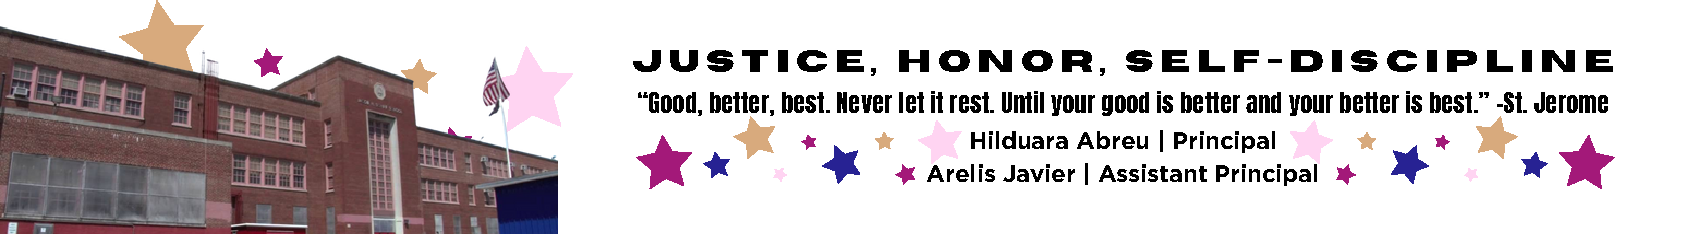
\includegraphics[width=8.8in,height=1.3in]{logo-1}}\end{picture}}
\fancyhead[C]{\setlength{\unitlength}{1in}\begin{picture}(5,0)\put(-1.9,-0.5){
\includegraphics[width=8.9in,height=1.3in]{logo-2}}\end{picture}}
\fancyhead[R]{\thepage}
\pagenumbering{gobble}

\begin{document}
\vspace*{0.01in}
Date: \href{https://www.ps192.org/apps/bbmessages/show_bbm.jsp?REC_ID=139439}{February 16, 2024}

Subject: \textbf{Bell Schedule}

A bell schedule specifies the start time and duration of one or more instructional periods on each day of a day pattern. A consistent daily schedule and step-by-step routines give children a predictable day. A Bell Schedule helps children:
\begin{itemize}
\item Feel in control of their environment
\item Feel safe, secure, and comfortable
\item Know what is happening now and what comes next
\item Know how to do an activity or task
\item Engage in learning
\end{itemize}

Just like adults, children feel more confident and secure when their daily activities are predictable and familiar.

\tcbuselibrary{skins}
\newtcolorbox{bluebox}[1][]{
  colback=blue!5!white,
  colframe=blue!75!black,
  fonttitle=\bfseries,
  coltitle=black,
  enhanced,
  attach boxed title to top center={yshift=-2mm},
  title=#1,
  boxed title style={colback=blue!50!white}
}
\newtcolorbox{greenbox}[1][]{
  colback=green!5!white,
  colframe=green!75!black,
  fonttitle=\bfseries,
  coltitle=black,
  enhanced,
  attach boxed title to top center={yshift=-2mm},
  title=#1,
  boxed title style={colback=green!50!white}
}
\newtcolorbox{redbox}[1][]{
  colback=red!5!white,
  colframe=red!75!black,
  fonttitle=\bfseries,
  coltitle=black,
  enhanced,
  attach boxed title to top center={yshift=-2mm},
  title=#1,
  boxed title style={colback=red!50!white}
}

\begin{bluebox}[PS 192 | Bell Schedule]
\begin{table}[H]
\centering
\begin{tblr}{
  colspec={|X|X|X|X|},
  row{1}={font=\bfseries\color{MacaroniandCheese},c},
  hlines,
  vlines,
  hline{1,10} = {-}{0.08em},
}
\textbf{Period} & \textbf{Start Time} & \textbf{End Time} & \textbf{Length} \\
1               & 08:00 AM            & 08:45 AM          & 45 minutes      \\
2               & 08:45 AM            & 09:30 AM          & 45 minutes      \\
3               & 09:30 AM            & 10:15 AM          & 45 minutes      \\
4               & 10:15 AM            & 11:05 AM          & 50 minutes      \\
5               & 11:05 AM            & 11:55 AM          & 50 minutes      \\
6               & 11:55 AM            & 12:40 PM          & 45 minutes      \\
7               & 12:40 PM            & 01:30 PM          & 50 minutes      \\
8               & 01:30 PM            & 02:15 PM          & 45 minutes
\end{tblr}
\end{table}
\end{bluebox}

With Justice, Honor, and Self-Discipline,


\includegraphics[width=0.2\textwidth]{hil_signature}

\textbf{Hilduara Abreu, Principal}

\textbf{The school of Joyful Learning!}

\href{www.ps192.org}{www.ps192.org}
\end{document}
